\documentclass[a4paper,12pt]{article}
\usepackage{amsmath}
\usepackage{amssymb}
\usepackage[polish]{babel}
\usepackage{polski}
\usepackage[utf8]{inputenc}
\usepackage{indentfirst}
\usepackage{geometry}
\usepackage{array}
\usepackage[pdftex]{color,graphicx}
\usepackage{subfigure}
\usepackage{afterpage}
\usepackage{setspace}
\usepackage{color}
\usepackage{wrapfig}
\usepackage{listings}
\usepackage{datetime}

\renewcommand{\onehalfspacing}{\setstretch{1.6}}

\geometry{tmargin=2.5cm,bmargin=2.5cm,lmargin=2.5cm,rmargin=2.5cm}
\setlength{\parindent}{1cm}
\setlength{\parskip}{0mm}

\newenvironment{lista}{
\begin{itemize}
  \setlength{\itemsep}{1pt}
  \setlength{\parskip}{0pt}
  \setlength{\parsep}{0pt}
}{\end{itemize}}

\newcommand{\linia}{\rule{\linewidth}{0.4mm}}

\definecolor{lbcolor}{rgb}{0.95,0.95,0.95}
\lstset{
    backgroundcolor=\color{lbcolor},
    tabsize=4,
  language=C++,
  captionpos=b,
  tabsize=3,
  frame=lines,
  numbers=left,
  numberstyle=\tiny,
  numbersep=5pt,
  breaklines=true,
  showstringspaces=false,
  basicstyle=\footnotesize,
  identifierstyle=\color{magenta},
  keywordstyle=\color[rgb]{0,0,1},
  commentstyle=\color[rgb]{0,0.5,0},
  stringstyle=\color{red}
  }

\begin{document}

\noindent
\begin{tabular}{|c|p{11cm}|c|} \hline
Grupa~4 & Katarzyna Kosiak i~Michał Folwarski & \ddmmyyyydate\today \tabularnewline
\hline
\end{tabular}

\section*{Zadanie~2 -- Rozmycie Gaussa w~MPI}
Program rozmywa zadane zdjęcie za pomocą algorytmu Gaussa z~maską o~wymiarach 5x5 korzystając z~zadanej liczby procesów.
Zrównoleglono rozmywanie rzędów pikseli zadanego zdjęcia:
\begin{lstlisting}
if (rank == 0) {
	if (numberOfProcesses == 1) {
	//oblicz w jednym watku
	} else {
	// podziel obraz na tyle blokow ile jest pozostalych watkow
	// kazdemu z watkow poza aktualnym wyslij jeden blok oraz informacje o jego rozmiarze
	// odbierz wszystkie bloki przefiltrowanego obrazu	 oraz ich rozmiary
	// poskladaj bloki do jednego obrazu
	}
} else {
	// odbierz blok obrazu
	// odbierz rozmiar bloku obrazu
	// przefiltruj otrzymany blok
	// wyslij blok przefiltrowanego obrazu oraz jego rozmiar do watku 0
}
\end{lstlisting}

Proces zerowy został uznany za nadzorujący całą operację filtrowania obrazu -- wykluczono go z~przetwarzania obrazu w~celu zwiększenia przejrzystości programu. Wątek zerowy rozsyła jednokrotnie równe bloki obrazu pozostałym procesom, dzięki czemu wszystkie wykonują tę samą ilość działań o nierosnącym poziomie trudności i~nie muszą niepotrzebnie czekać na kolejne wiadomości od procesu zerowego. To rozwiązanie spełnia nasze oczekiwania pod względem prostoty oraz skuteczności.

\begin{figure}[!hbtp]
  \centering
  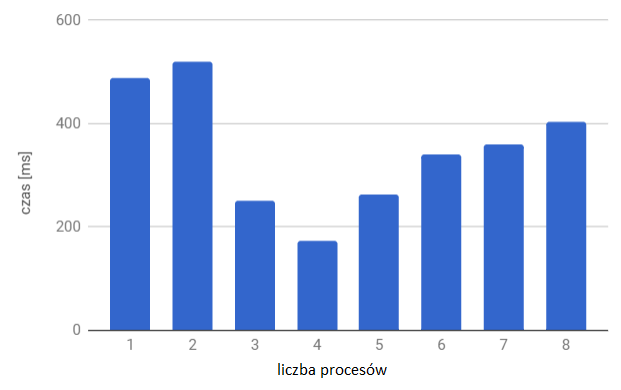
\includegraphics[width=0.8\textwidth]{wykres.png}
  \caption{Zależność czasu wykonania zadania od ilości procesów}
\end{figure}
Zamieszczony wykres na rysunku~1 pokazuje zależność czasu działania programu od liczby procesów dla przykładowego obrazu o~rozmiarze boku około 1500px na komputerze z~czterema procesorami.

Najkrótszy czas osiągnięto podczas zrównoleglenia na liczbę procesów równą liczbie procesorów. Dalsze zwiększanie liczby procesów może tylko pogorszyć czas, ponieważ musi zostać poświęcony dodatkowy czas na przełączanie kontekstu dla poszczególnych procesów na współdzielonych procesorach.

Czas wykonania zadania dla dwóch procesów jest większy niż dla jednego ponieważ tylko jeden z~nich wykonuje właściwe obliczenia, podczas gdy wątek zerowy (pełniący rolę administratora) czeka na odebranie wiadomości z~przefiltrowanym obrazem.

Kolejny wykres (Rysunek~2) pokazuje dodatkowo, że nie nastąpiło idealnie trzykrotne przyspieszenie -- wynika to z~faktu, że przydzielanie zadań procesom i~zarządzanie nimi także wymaga zasobów oraz tego, że wątek zerowy pełni rolę nadzorującą i~nie wykonuje obliczeń związanych z~filtrowaniem obrazu.

\begin{figure}[!hbtp]
  \centering
  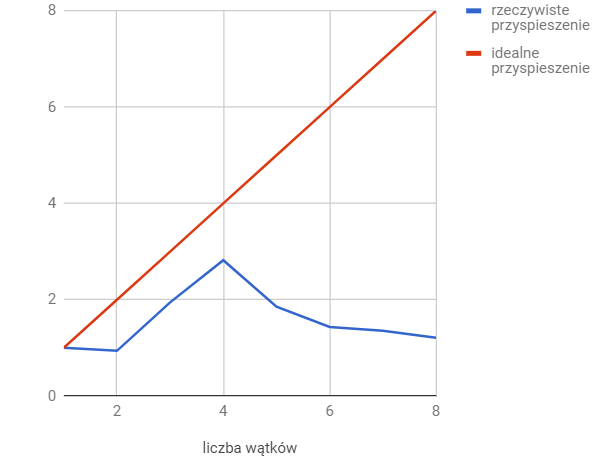
\includegraphics[width=0.8\textwidth]{wykres2.png}
  \caption{Zależność przyspieszenia wykonywania zadania od ilości procesów w~stosunku do niezrównoleglonego zadania}
\end{figure}

\subsubsection*{Wnioski }
Zadanie udało się wykonać -- dokonano zrównoleglenia obliczeń. Wykorzystanie MPI w~tym przypadku (niezależne od siebie obliczenia o~tej samej złożoności) było skuteczne. Komunikacja między procesami została osiągnięta poprzez wykorzystanie systemu wysyłania i~odbierania wiadomości. W~stosunku do rozwiązania z~wykorzystaniem OpenMP, użycie MPI jest trudniejsze -- wymaga podjęcia decyzji o~roli każdego z procesów, jednak dzięki temu można lepiej sterować programem.
\end{document}
